\section{Hintergrund}
\label{Hintergrund}
Der Fußschalter soll in einer komplexen Umgebung aus Messwerkzeug und Computer agieren, weshalb in diesem Kapitel zum Verständnis wichtige Hintergrundinformationen gegeben werden sollen. Es wird \ac{BLE} vorgestellt, dass die Grundtechnologie für den Informationsaustausch zwischen Fußschalter und dem Messwerkzeug darstellt, sowie die \ac{HCT}-Plattform und das \ac{HCT}-Protokoll auf dem sie aufbaut.

\subsection{Bluetooth Low Energy}
Bluetooth Low Energy ist eine Funktechnologie, die in Hinsicht auf einen sehr geringen Energieverbrauch entwickelt wurde. Sie arbeitet im 2.4GHz unlicensed ISM frequency band. (\cite[]{Bluetooth_Wireless_Technology}) \ac{BLE} findet hauptsächlich Verwendung darin, eine einfache ``kabellose Verbindung zwischen einem und Audioendgeräten'' herzustellen, sowie die ``Anbindung von kabellosen Tastaturen und anderen Eingabegeräten an Notebooks, PCs und Smartphones'' zu ermöglichen. (\cite[S. 339]{Grundkurs_mobile_Kommunikation})\\
Die Übertragung von gerätespezifischen Daten, wie die derzeit gemessen Temperatur bei einem digitalen Thermometer, erfolgt dabei über das \ac{GATT}. Es definiert Charakteristiken und ihre Attribute. Sie werden während des Verbindungsaufbaus übermittelt und ein Server kann sich auf Charakteristik anmelden, sodass er über eine Änderung der Attribute vom Client selbstständig notifiziert wird, was als Subscription bezeichnet wird. Andernfalls kann er direkt über einen Request die Werte einer Charakteristik anfordern. Mehrere Charakteristiken werden in einem Service zusammengefasst.(\cite[S. 1459]{Bluetooth_Core_Specification})(\cite[]{Overview_and_Evaluation_of_BLE}) Der Protokoll Stack von Bluetooth hält sich ``lose an das 7 Schichten OSI Modell'' (\cite[S. 347]{Grundkurs_mobile_Kommunikation}).\\
Innerhalb einer Verbindung über Bluetooth werden den Geräten verschiedene Rollen zugeordnet. Das Gerät das den Verbindungsaufbau initiert hat wird als das ``Central'' bezeichnet und verarbeitet die Daten des ``Peripheral''. Das Peripheral ist dabei meist ein Gerät, welches streng limitiert durch seinem ihm zur Verfügung stehenden Ressourcen ist und stellt seinem Daten dem Central zur Verfügung. Wird ein digitals Thermometer mit einem Handy verbunden um die Temperatur abzulesen, ist somit das Therometer das Peripheral und das Handy das Central. Neben den Rollen Central und Peripheral, gibt es weiterhin die Rollen ``Broadcaster'' und ``Observer'', diese haben jedoch für diese Arbeit kein Bedeutung (\cite[S. 1246]{Bluetooth_Core_Specification}).\\
Bei den Werkzeugen der Hoffmann Group wurde sich für \ac{BLE} als Verbindungsmedium entschieden, da den Hand- und Messwerkzeugen, aufgrund ihres Formafaktors und nicht kabelgebundenheit, nur begrenzte Batteriespeicherkapazitäten zu Verfügung stehen.

\subsection{HCT-Plattform}
Um die Digitalisierung der Messergebnisse dem Anwender so einfach wie möglich zu gestalten, setzt die Hoffmann Group mit der \ac{HCT}-Plattform darauf, die Digitalisierung der durchgeführten Arbeitsschritte als einen festen Bestandteil in ihr Werkzeug zu integrieren. Diese sind zum Stand dieser Arbeit: 
\begin{itemize}
	\item Drehmomentschlüssel
	\item Messschieber bzw. Messuhren
	\item Drehmomentprüfgerät
	\item Bügelmessschrauben
\end{itemize}
Sie stellen dem Anwender die Daten der Messungen in verschiedener Weise zu Verfügung. Zum Einen können die Geräte als ein \ac{HID} über \ac{BLE} mit dem Computer verbunden werden. Sie simulieren dann eine über Bluetooth verbundene Tastatur über die, die Messergebnisse als Tastendrücke serialisiert werden. Das Messergebnis kann dann in einem Texteditor oder Excel aufgefangen werden. Des weiteren erzeugen die Drehmomentschlüssel und das Drehmomentprüfgerät eine \ac{CSV}-Datei, in der alle durchgeführten Messungen mit einer großen Anzahl an zusätzlichen Daten gespeichert werden. Wird das Gerät über \ac{USB} mit dem Computer verbunden, zeigt es sich als \ac{MSC}-Device und die Datei kann per Drag-and-drop auf den Computer kopiert werden. Eine weitere Möglichkeit die durchgeführten Messungen zu digitalisieren, ist mithilfe der \ac{HCT}-Windows-App. Diese erfordert zusätzlich zur frei verfügbaren Software einen speziellen Dongle der zum Verbinden der Geräte benötigt wird. Sie werden ebenfalls über \ac{BLE} verbunden und sprechen über \ac{BLE} das firmeneigene \ac{HCT}-Protokoll. Die Windows-App bietet zahlreiche Möglichkeiten die Messdaten zu digitalisieren und den Produktionsprozess zu optimieren. Es können Schraubfälle in der App angelegt werden und mit Bildern hinterlegt werden. Die Seriennummer von Werkstücken kann automatisch mit dem dazugehörigen Messwert verlinkt werden und \ac{CAQ}-Software kann über einen virtuelle COM-Port angebunden werden. Die \ac{HCT}-Windows-App unterstützt derzeit lediglich die Drehmomentschlüssel, jedoch ist die Einbindung der restlichen \ac{HCT}-Geräte in Entwicklung. Der Fußschalter und der Dongle nehmen dabei eine ähnliche Position, jedoch mit geringerem Funktions- und Userinterfaceumfang, wie die Windows-App ein. Der letzte Baustein der \ac{HCT}-Plattform ist die \ac{HCT}-Mobile-App, sie ist ebenfalls frei erhältlich und erleichtert vorallem die Bedienung des Geräts, zum Beispiel bei Arbeitsschritten bei denen das Display des Werkzeugs für den Anwender nicht sichtbar ist.

\begin{figure}[H] 
	\centering
	\includegraphics[width=\textwidth]{figures/Ökosystem.png}
	\caption{Schematische Zeichnung der \ac{HCT}-Plattform}
\end{figure}

\subsection{HCT-Protokoll}
Der \ac{HCT}-Plattform liegt das firmeneigene \ac{HCT}-Protokoll zugrunde. Es stellt sicher, dass alle Geräte der \ac{HCT}-Plattform stets kompatibel zu einander sind. Es ist ein binäres Protokoll, dass entwickelt wurde um über \ac{BLE} gesprochen zu werden und stellt ein virtuelles Speichermodel der Geräte da. Dabei besitzten Werkzeuge unterschiedlicher Produktreihen und Hersteller jeweils verschiedene Speichermodelle. Über ``READ'' und ``WRITE'' Befehle auf die Speicheradressen kann dann der interne Zustand des Werkzeug abgefragt und verändert werden. Siehe \ref{appendix:HCT-Protocol-Description}. So können auch komplexe Operationen effizient über \ac{BLE} durchgeführt werden. Der virtuelle Speicher ist dabei in Datenblöcken unterteilt, welche die Daten in logische Gruppen zusammenfassen. Die Datenblöcke stellen die Referenzadressen zu spezifischen Dateneinträgen dar. In Abbildung 2 ist ein Auszug aus dem Speichermodell der Messuhren bzw. Messschieber mit den erwähnten Datenblöcken und spezifischen Dateneinträgen zu sehen. Zudem stehen automatisierte Tools zur Verfügung mit deren Hilfe das Framework, welche die Kommunikation über das HCT-Protokoll abstrahiert, um die Speichermodelle neu eingeführter Werkzeuge erweitert werden kann. Dieses Framework trägt den internen Name ``nrf\_Base'' und stellt die Anwendungsschicht im Bluetooth-Stack dar.

\begin{figure}[H] 
	\centering
	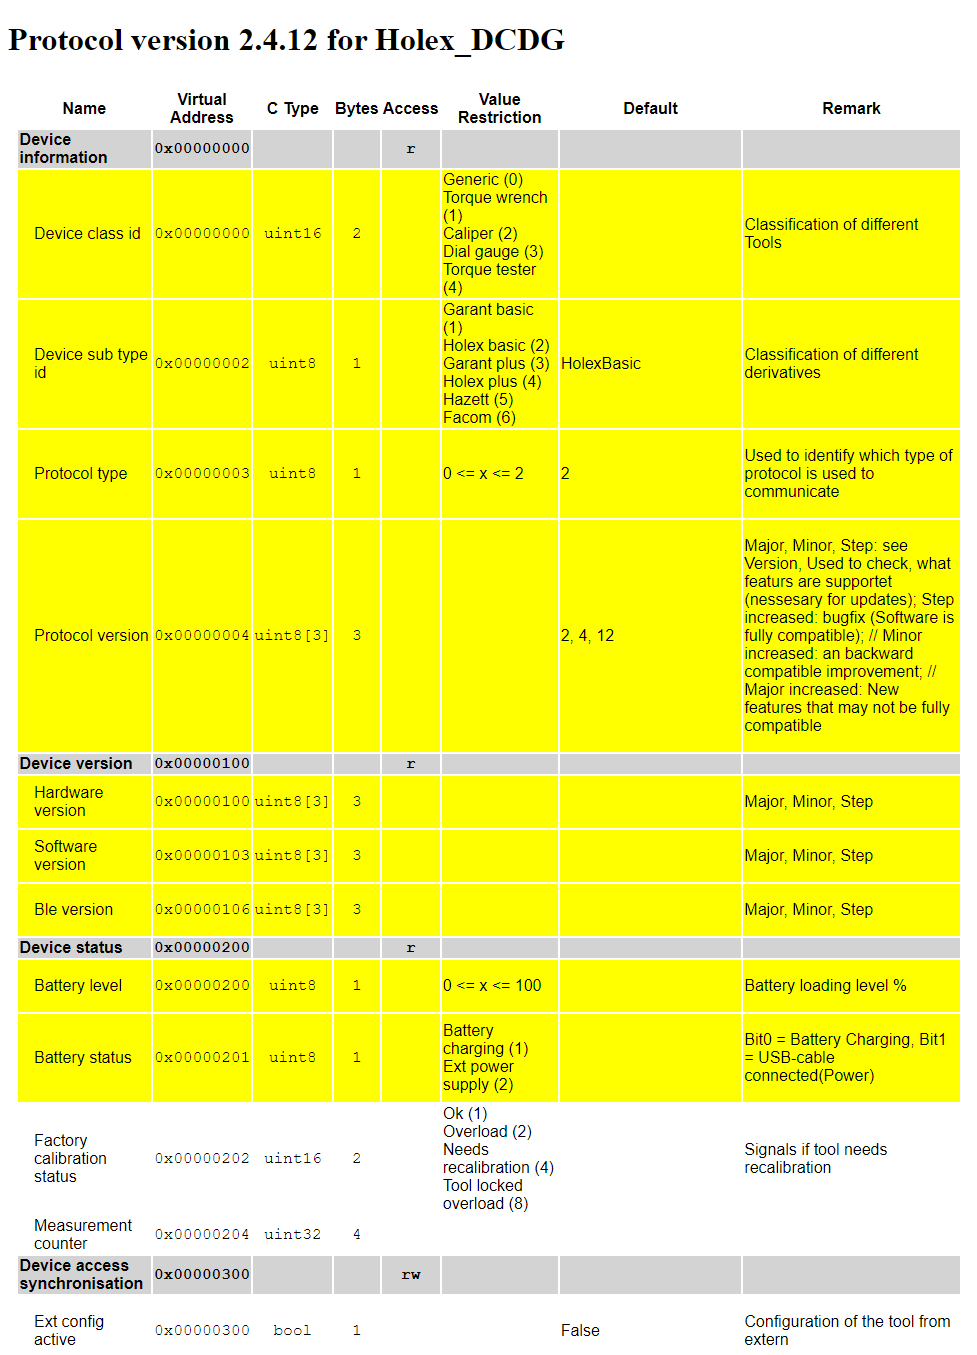
\includegraphics[width=\textwidth]{figures/HCT_Protocol_DCDG.png}
	\caption{Auszug aus dem virtuellen Speichermodell für Messuhren und Messschieber}
\end{figure}